% 角动量定理 角动量守恒
% 角动量|角动量定理|角动量守恒|力矩|牛顿第二定律

\pentry{角动量定理\ 角动量守恒(单个质点)\upref{AMLaw1}, 牛顿第三定律\upref{New3}}
\textbf{角动量定理}可以表示为
\begin{equation}\label{AMLaw_eq1}
\dv{\bvec L}{t} = \bvec \tau
\end{equation}
即系统的角动量对时间的变化率等于所受外力的合力矩.系统可以包括任意选定的若干物体.

\subsection{推导}
推导可类比动量定理\upref{PLaw}.我们已经知道单个质点的角动量,而任何物体都可以划分成若干足够小的微元,每个微元可以看成一个质点.令第 $i$ 个质点的位矢为 $\bvec r_i$, 角动量为 $\bvec L_i$,力矩为 $\bvec \tau_i$,单个质点的角动量定理\upref{AMLaw1} 为
\begin{equation}
\dv{\bvec L_i}{t} = \bvec \tau_i = \bvec \tau_i^{in} + \bvec \tau_i^{out}
\end{equation}
其中 $\bvec \tau_i^{in}$ 和 $\bvec \tau_i^{out}$ 为质点 $i$ 受到的系统内其他质点的力矩和来自系统外的力矩.将该式对所有 $i$ 求和,得到总角动量 $\bvec L$ 变化率
\begin{equation}
\dv{\bvec L}{t} =\sum_i\dv{\bvec L_i}{t} = \sum_i\bvec \tau_i^{in} + \sum_i\bvec \tau_i^{out}
\end{equation}
现在我们只需证明质点系的合内力矩为零即可
\begin{equation}
\sum_i\bvec \tau_i^{in} = \sum_i \qty(\bvec r_i\cross\sum_j^{j\ne i}\bvec F_{j\to i}) = \sum_{i,j}^{i\ne j} \bvec r_i\cross\bvec F_{j\to i}
\end{equation}
其中 $\bvec F_{j\to i}$ 是质点 $j$ 对质点 $i$ 的力.现在只考虑任意两个质点 $k$ 和 $l$,在求和中的贡献为
\begin{equation}
\bvec r_k\cross\bvec F_{l\to k} + \bvec r_l\cross\bvec F_{k\to l} \equiv \bvec \tau_{l\to k}+ \bvec \tau_{k\to l}
\end{equation}
即 $k$ 对 $l$ 的力矩加 $l$ 对 $k$ 的力矩(两质点的和内力矩).所以若能证明任意两质点的和内力矩为零,则质点系的合内力矩为零.

我们先来看几何证明.如\autoref{AMLaw_fig1}, 根据定义, 力矩的大小等于力的模长乘以力臂的长度\upref{Torque}, 而一对相互作用力的大小相同, 又由于二者共线, 力臂也重合, 所以两个力矩大小相等. 但是两个力矩的方向一个是顺时针(指向纸内), 一个是逆时针(指向纸外), 所以两力矩互相抵消, 相加为零.

\begin{figure}[ht]
\centering
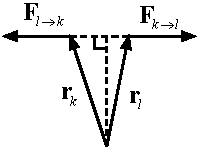
\includegraphics[width=3.7cm]{./figures/AMLaw1.pdf}
\caption{两质点的相互作用力对总力矩贡献为零}\label{AMLaw_fig1}
\end{figure}

再在看代数的方法:我们先沿着两质点的连线写出相互作用力 $\bvec F_{l\to k} = \alpha(\bvec r_k - \bvec r_l)$, $\bvec F_{k\to l} = \alpha(\bvec r_l - \bvec r_k)$,直接计算两力矩和得
\begin{equation}
\bvec r_k \cross (\bvec r_k - \bvec r_l)\alpha + \bvec r_l \cross (\bvec r_l - \bvec r_k)\alpha = 0
\end{equation}
证毕.

\begin{example}{单车轮与转椅实验}
小明开始时坐在静止的转椅上, 两手握住一个单车轮的轴的两端, 单车轮在水平面上转动. 这时小明将单车轮上下翻转(仍保持转动), 问小明与转椅会如何转动?

假设开始时车轮的角动量向上, 那么翻转后车轮的角动量向下, 即角动量增量向下. 由于角动量守恒,小明的身体和转椅的角动量必须有一个向上的增量, 所以转椅最后的旋转方向与轮子开始时的旋转方向相同.
\end{example}

\begin{example}{陀螺的进动}\label{AMLaw_ex2}
\begin{figure}[ht]
\centering
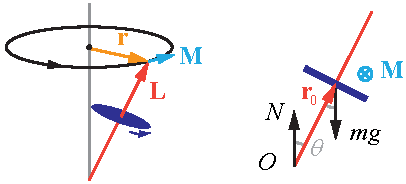
\includegraphics[width=7cm]{./figures/AMLaw2.pdf}
\caption{陀螺的进动}\label{AMLaw_fig2}
\end{figure}
如\autoref{AMLaw_fig2}(左), 陀螺旋转时, 若它的轴与竖直方向有一定倾角, 轴会绕一个竖直轴缓慢旋转, 这种现象被称为\textbf{进动}. 为了便于分析, 我们先假设陀螺进动的角速度比陀螺自转的角速度要慢得多. 这样, 我们就可以认为陀螺的角动量 $\bvec L$ 与陀螺的轴平行. 显然, 陀螺的进动意味着陀螺的角动量变化率 $\dv*{\bvec L}{\bvec t}$ 的方向始终垂直于图中 $\bvec r$ 和 $\bvec L$ 所在的平面. 根据角动量定理, 陀螺所受的力矩 $\bvec \tau$ 也具有同样的大小和方向.

那么这个力矩是如何产生的呢? 我们对陀螺进行受力分析如\autoref{AMLaw_fig2}(右), 要计算陀螺所受力矩, 我们取轴的底端为原点, 假设陀螺的轴没有质量, 则地面对陀螺的支持力 $N$ 产生的力矩为零, 而重力产生的力矩为 $\bvec \tau = \bvec r_0 \cross (m\bvec g)$, 其大小为 $mgr_0\sin\theta$, 方向垂直纸面向里, 恰好符合陀螺进动的要求.

比较违反直觉的地方在于, 陀螺受到的重力是延使陀螺倾倒的方向施加的, 然而陀螺不但丝毫不会倾倒(如果不计摩擦), 反而其重心会向着与重力垂直的方向移动.
\end{example}

% 未完成: 例: 双转盘的陀螺不能保持平衡